\documentclass[12pt, twoside]{article}
\usepackage[francais]{babel}
\usepackage[T1]{fontenc}
\usepackage[latin1]{inputenc}
\usepackage[left=5mm, right=5mm, top=3mm, bottom=3mm]{geometry}
\usepackage{float}
\usepackage{graphicx}
\usepackage{array}
\usepackage{multirow}
\usepackage{amsmath,amssymb,mathrsfs}
\usepackage{soul}
\usepackage{textcomp}
\usepackage{eurosym}
 \usepackage{variations}
\usepackage{tabvar}


\pagestyle{empty}

\begin{document}



\section*{\center{Devoir maison 3}}

\begin{center}
\fbox{
\begin{minipage}{19cm}
\textit{Devoir � rendre sur feuille grand format pour le \ul{mercredi 6 janvier
2015}. La justification et la \textbf{r�daction} seront prises en
 compte dans le bar�me.}
 \end{minipage}
} 
\end{center}

 
\bigskip

\textbf{\ul{Exercice 1}} \textit{(4 points)}

\begin{tabular}{cc}
\begin{minipage}{9cm}

En utilisant les informations port�es sur la figure:


\begin{enumerate}
  \item Calculer MN.
  \item En d�duire BC.
\end{enumerate} 
\end{minipage}
&
\begin{minipage}{9cm}
\begin{center}
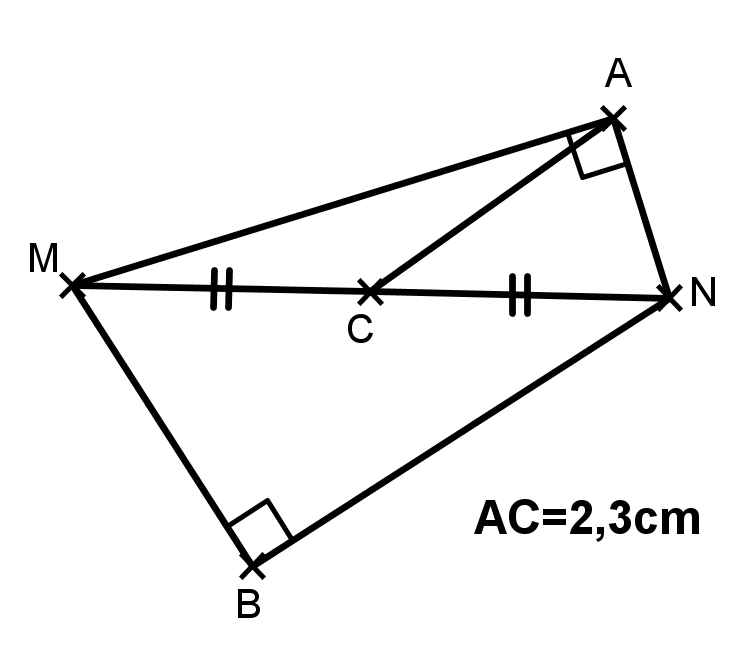
\includegraphics[width=4cm]{images/ex2bis.png}
\end{center}

\end{minipage}
\end{tabular}

\bigskip

\textbf{\ul{Exercice 2}} \textit{(3,5 points)}


\begin{tabular}{cr} 
\begin{minipage}{11cm}

Construire un point P tels que les triangles ABP et CDP soient rectangles en P.
Justifier votre r�ponse.

\enskip

(\textit{La construction se fera sur la photocopie et les explications seront
not�es sur votre feuille.})


\end{minipage}
&
\begin{minipage}{7cm}
\begin{center}

\includegraphics[width=65mm]{images/ex4.png}
\end{center}
\end{minipage} 
\end{tabular}

\bigskip

\textbf{\ul{Exercice 3}} \textit{(4,5 points)}


\enskip

 Soit [IJ] un segment de longueur 8cm. $\mathcal{C}$
est le cercle de diam�tre [IJ]. Le point K appartient au cercle $\mathcal{C}$
et v�rifie JK=3,5cm.



\begin{enumerate}
  \item Faire la figure.
  \item D�montrer que le triangle IJK est rectangle en K.
  \item Calculer IK (on donnera le r�sultat arrondi au mm). Justifier votre
  r�ponse.
\end{enumerate}

\bigskip


\textbf{\ul{Exercice 4}} \textit{(4 points)}

\enskip

\begin{enumerate}
  \item Traduire les phrases suivantes par un calcul:
  
  \begin{enumerate}
    \item [a)]Le produit de la somme de -3 et de -5 par la diff�rence de 6 et de
    -8.
    \item [b)]Le quotient de -75 par la diff�rence de 8 et de 14.
   
\end{enumerate}
\item Traduire les expressions math�matiques par des phrases:
\quad a) $25+7 \times (-2)$ \qquad \qquad 
 b) $\dfrac{4-(-6)}{(-3) \times (-2)}$ 

\end{enumerate} 

\bigskip

\textbf{\ul{Exercice 5}} \textit{(2 points)}

\enskip

Recopier et ajouter si n�cessaire des parenth�ses pour que ces �galit�s soient
vraies.

\begin{enumerate}
 \item [a)] \thinspace $5 - 4 \times 3 + 2 = 5$  

 \item [b)] \thinspace $5 - 4 \times 3 + 2 = -15$  


 \item [c)] \thinspace $5 - 4 \times 3 + 2 = -9$

\end{enumerate}

\bigskip


\textbf{\ul{Exercice 6}} \textit{(2 points)}

\enskip

a est un nombre positif quelconque. Quel est le signe de l'expression $a^2
\times (-a)^3$? Expliquez votre d�marche.
\end{document}
